%%%%%%%%%%%%%%%%%%%%%%%%%%%%%%%%%%%%%%%%%%%%%%%%%%%%%%%%%%%%%%%%%%%%%%%%%%%%
% AGUtmpl.tex: this template file is for articles formatted with LaTeX2e,
% Modified March 2009
%
% This template includes commands and instructions
% given in the order necessary to produce a final output that will
% satisfy AGU requirements.
%
% PLEASE DO NOT USE YOUR OWN MACROS
%
% For more information on using the AGUTeX macro package,
% see agudocs.tex or agudocs.pdf
%
%%%%%%%%%%%%%%%%%%%%%%%%%%%%%%%%%%%%%%%%%%%%%%%%%%%%%%%%%%%%%%%%%%%%%%%%%%%%
%
% All questions should be e-mailed to author.help@agu.org.
%
%%%%%%%%%%%%%%%%%%%%%%%%%%%%%%%%%%%%%%%%%%%%%%%%%%%%%%%%%%%%%%%%%%%%%%%%%%%%
%
% Step 1: set the \documentclass
%
% The three options for article format are: two-column (default),
% draft, for initial article submission; and galley for narrow
% single columns.
%
% PLEASE USE THE DRAFT OPTION TO SUBMIT YOUR PAPERS
% The draft option produces double spaced output
%
% Choose the journal abbreviation for the journal you are
% submitting to:

% jgrga JOURNAL OF GEOPHYSICAL RESEARCH
% gbc   GLOBAL BIOCHEMICAL CYCLES
% grl   GEOPHYSICAL RESEARCH LETTERS
% pal   PALEOCEANOGRAPHY
% ras   RADIO SCIENCE
% rog   REVIEWS OF GEOPHYSICS
% tec   TECTONICS
% wrr   WATER RESOURCES RESEARCH
% gc    GEOCHEMISTRY, GEOPHYSICS, GEOSYSTEMS

% (If you are submitting to a journal other than jgrga,
% substitute the initials of the journal for "jgrga" below)

%\documentclass[draft,grl]{agutex}
\documentclass[grl]{agutex}
\bibliographystyle{agufull08}

%%%%%%%%%%%%%%%%%%%%%%%%%%%%%%%%%%%%%%%%%%%%%%%%%%%%%%%%%%
%%%% optional article formats author might want to use

% To produce a galley version:
% \documentclass[galley,jgrga]{AGUTeX}

% To produce a two columned version:
% \documentclass[jgrga]{AGUTeX}

%%%%%%%%%%%%%%%%%%%%%%%%%%%%%%%%%%%%%%%%%%%%%%%%%%%%%%%%%%%%%%%%%%%%%%%%%
% OPTIONAL:
% To print your article using PostScript fonts, uncomment this:
% \usepackage{agu-ps}
% You many need to edit the top of agu-ps to use the names of the PS
% fonts on your system.

%%%%%%%%%%%%%%%%%%%%%%%%%%%%%%%%%%%%%%%%%%%%%%%%%%%%%%%%%%%%%%%%%%%%%%%%%
% OPTIONAL:
% To Create numbered lines:

% If you don't already have lineno.sty, you can download it from
% http://www.ctan.org/tex-archive/macros/latex/contrib/ednotes/
% (or google lineno.sty ctan), available at TeX Archive Network (CTAN).
% Take care that you always use the latest version.

% To activate the commands, uncomment \usepackage{lineno}
% and \linenumbers*[1]command, below:

% \usepackage{lineno}
% \linenumbers*[1]

%%%%%%%%%%%%%%%%%%%%%%%%%%%%%%%%%%%%%%%%%%%%%%%%%%%%%%%%%%%%%%%%%%%%%%%%%
% Figures and Tables
%

% When submitting articles through the GEMS system:
% COMMENT OUT ANY COMMANDS THAT INCLUDE GRAPHICS.
% (See FIGURES section near the end of the file)


%  Figures and Tables should be placed at the end of the article,
%  after the references.
%
%  Uncomment the following command to include .eps files
%  (comment out this line for draft format):
\usepackage{graphicx}
\usepackage{multirow}  % DR Needed to setup figure 1 - must comment out for final version..
%
%    Uncomment the following command to allow illustrations to print
%    when using Draft:
\setkeys{Gin}{draft=false}
%
% Substitute one of the following for [dvips] above
% if you are using a different driver program and want to
% proof your illustrations on your machine:
%
% [xdvi], [dvipdf], [dvipsone], [dviwindo], [emtex], [dviwin],
% [pctexps],  [pctexwin],  [pctexhp],  [pctex32], [truetex], [tcidvi],
% [oztex], [textures]
%
% See how to enter figures and tables at the end of the article, after
% references.
%
%% ------------------------------------------------------------------------ %%
%
%  ENTER PREAMBLE
%
%% ------------------------------------------------------------------------ %%

% Author names in capital letters:
\authorrunninghead{ROBINSON ET AL.}

% Shorter version of title entered in capital letters:
\titlerunninghead{LOCATING POORLY RECORDED EARTHQUAKES USING CODA WAVES}

% Author mailing address: please repeat this command for
% each author and alphabetize authors:


\authoraddr{D. J. Robinson,
Research School of Earth Sciences, Australian National University, Canberra, ACT, 0200, Australia.
 (david.robinson@anu.edu.au) and
Risk Research Group, Geoscience Australia, GPO Box 378, Canberra, ACT, 2601, Australia.
 (david.robinson@ga.gov.au)}

\authoraddr{M. Sambridge,
Research School of Earth Sciences, Australian National University, Canberra, ACT, 0200, Australia.
 (malcolm.sambridge@anu.edu.au)}

\authoraddr{R. Snieder,
Center for Wave Phenomena and Department of Geophysics, Colorado School of Mines,
    Golden CO 80401, USA.
 (rsnieder@mines.edu)}

\authoraddr{P. Cummins,
Research School of Earth Sciences, Australian National University, Canberra, ACT, 0200, Australia.
 (phil.cummins@anu.edu.au) and
Risk Research Group, Geoscience Australia, GPO Box 378, Canberra, ACT, 2601, Australia.
 (phil.cummins@ga.gov.au)}

\authoraddr{J. Dawson,
Earth Monitoring Group,Geoscience Australia, GPO Box 378, Canberra, ACT, 2601, Australia.
 (john.dawson@ga.gov.au)}

%\authoraddr{J. R. McConnell, Division of Hydrologic
%Sciences, 123 Main Street, Desert Research Institute, Reno, NV
%89512, USA.}

%\authoraddr{E. Mosley-Thompson, Department of Geography,
%Ohio State University, 123 Orange Boulevard, Columbus, OH 43210,
%USA.}

%\authoraddr{R. Williams, Department of Space Sciences, University of
%Michigan, 123 Brown Avenue, Ann Arbor, MI 48109, USA.}

\begin{document}

%% ------------------------------------------------------------------------ %%
%
%  TITLE
%
%% ------------------------------------------------------------------------ %%


\title{Accurate relative location using coda waves of a poorly recorded cluster of earthquakes near Kalannie, Western Australia}
%
% e.g., \title{Terrestrial ring current:
% Origin, formation, and decay $\alpha\beta\Gamma\Delta$}
% You may use \\ to break the title over several lines.

%% ------------------------------------------------------------------------ %%
%
%  AUTHORS AND AFFILIATIONS
%
%% ------------------------------------------------------------------------ %%


%Use \author{\altaffilmark{}} and \altaffiltext{}

% \altaffilmark will produce footnote;
% matching altaffiltext will appear at bottom of page.
% May use \\ to start a new line.

\authors{D. J. ROBINSON, \altaffilmark{1,} \altaffilmark{2}
M. SAMBRIDGE,  \altaffilmark{1}
R. SNIEDER, \altaffilmark{3}
P. CUMMINS \altaffilmark{1,} \altaffilmark{2}
AND J. DAWSON \altaffilmark{4}}
%E. Mosley-Thompson, \altaffilmark{2} R. Williams, \altaffilmark{3}
%and J. R. McConnell\altaffilmark{4}}

\altaffiltext{1}{Research School of Earth Sciences, The Australian National University}

\altaffiltext{2}{Risk Research Group, Geoscience Australia}

\altaffiltext{3}{Center for Wave Phenomena and Department of Geophysics, Colorado School of Mines}

\altaffiltext{4}{Earth Monitoring Group, Geoscience Australia}

%\altaffiltext{1}{Department of Hydrology and Water Resources,
%University of Arizona, Tucson, Arizona, USA.}

%\altaffiltext{2}{Department of Geography, Ohio State University,
%Columbus, Ohio, USA.}

%\altaffiltext{3}{Department of Space Sciences, University of
%Michigan, Ann Arbor, Michigan, USA.}

%\altaffiltext{4}{Division of Hydrologic Sciences, Desert Research
%Institute, Reno, Nevada, USA.}

%% ------------------------------------------------------------------------ %%
%
%  ABSTRACT
%
%% ------------------------------------------------------------------------ %%

% >> Do NOT include any \begin...\end commands within
% >> the body of the abstract.

\begin{abstract}
(Type abstract here)
\end{abstract}

%% ------------------------------------------------------------------------ %%
%
%  BEGIN ARTICLE
%
%% ------------------------------------------------------------------------ %%

% The body of the article must start with a \begin{article} command
%
% \end{article} must follow the references section, before the figures
%  and tables.

\begin{article}

%% ------------------------------------------------------------------------ %%
%
%  TEXT
%
%% ------------------------------------------------------------------------ %%

\section{Introduction}
\begin{itemize}
\item South West Seismic Zone (SWSZ) - one of Australia's most active source zones
\item Poor station coverage makes accurate location difficult
\item Kalannie earthquake cluster (figure \ref{fig:-Kalannie-map}(a))
\item \citet{dr_Dawson08a} composite mechanism (ref table \ref{tab-Dawson-Kalannie-results})
\item Validity of composite mechanism assumes overlapping rupture on the same fault - we demonstrate that
assumption holds despite the poor station coverage
\end{itemize}

\section{Methodology}
\begin{itemize}
\item Compute Kalannie event sizes (Table \ref{tab:Kalannie-eventsizes}) and comment on location
accuracy required to demonstrate that events are overlapping
\item Relative location with a few stations - use the coda
\item CWI separation (\citealp{dr_Snieder05a}; \citealp{dr_Snieder06a})
\item Possible to get separation estimate with a single station (e.g. \citealp{dr_Robinson07b})
\item \textbf{ref Paper1} - formulates CWI probabilistically for a pair of events - must comment on wavelength normalisation
\item \textbf{ref Paper2} - formulation of the joint posterior, misfit function $L$ and minimization by optimisation.
\item Problem with optimisation approach is that it gives a single solution only and can get trapped in
local minima. We use Markov-Chain Monte-Carlo (MCMC) here which allows a complete assessment of uncertainty.
This is only possible because of the small number of events considered.
\item \textbf{Malcolm and Roel - there is potentially a large number of equations to show here. I propose that we keep
the number of equations as small as possible and refer readers to the other papers and the thesis for details. Any
thoughts?}
\end{itemize}


\section{Results}

\begin{itemize}
\item Discuss waveforms, first arrival similarity and filtering between 1 and 2\,Hz (Figure \ref{fig:-Kalannie-map}(b))
\item We only have access to data from 3 stations MORW, BLDU and KLBR (Figure \ref{fig:-Kalannie-map}(a))
\item Application of CWI on event pairs (Figure \ref{fig:-Kalannie-map}(b))
\item Computation of CWI based pairwise separation posteriors (Figure \ref{fig:Kalannie-CWI-Posteriors})
\item Compare MCMC results (Expected Value and standard error) to optimisation solution (Table \ref{tab:Kalannie-InversionRes})
\item MCMC in more detail: 1D marginals, covariance and correlation (Figure \ref{fig:Kalannie-CWI-NAB-1Dmarginals})
\item MCMC in more detail: example 2D marginal (Figure \ref{fig:Kalannie-2Dmarginals_param23}).
Shows that events 1 and 2 are close but not co-located.
\item Discuss the separation estimates which incorporate CWI from all pairs (e.g. Table \ref{tab:-KalannieRes-separations})
\end{itemize}

\section{Conclusions}
\begin{itemize}
\item The power of CWI when limited stations available
\item Advantage of the MCMC inversion approach (i.e. detailed picture of uncertainty). Disadvantage that it
is computationally expensive (ref \textbf{Paper2} for optimisation approach with more events).
\item Demonstration that the events are close but not co-located. Consistent with hypothesis that the
four ruptures overlap on the same fault.
\end{itemize}




%%% End of body of article:

%%%%%%%%%%%%%%%%%%%%%%%%%%%%%%%%
%% Optional Appendix goes here
%
%%%%%%%%%%%%%%%%%
% Geophysical Research Letters only allows an appendix without a letter.
%% You can get this result with
%  \section*{Appendix}
%  or
%  \section*{Appendix: Title}
%%%%%%%%%%%%%%%%%
%
% \appendix resets counters and redefines section heads
% but doesn't print anything.
% After typing  \appendix
%
% \section{Here Is Appendix Title}
% will print
% Appendix A: Here Is Appendix Title
%
% \section*{Appendix}
% will print
% Appendix
%
% \section*{Appendix: Here Is Appendix Title}
% will print
% Appendix: Here Is Appendix Title
%
% For only 1 appendix \appendix \section{Appendix} is preferred.
% which will print
% Appendix A

%%%%%%%%%%%%%%%%%%%%%%%%%%%%%%%%%%%%%%%%%%%%%%%%%%%%%%%%%%%%%%%%
%
% Optional Glossary or Notation section, goes here
%
%%%%%%%%%%%%%%
% Glossary only allowed in Reviews of Geophysics
% \section*{Glossary}
% \paragraph{Term}
% Term Definition here
%
%%%%%%%%%%%%%%
% Notation -- End each entry with a period.
% \begin{notation}
% Term & definition.\\
% Second Term & second definition.
% \end{notation}
%%%%%%%%%%%%%%%%%%%%%%%%%%%%%%%%%%%%%%%%%%%%%%%%%%%%%%%%%%%%%%%%
%
%  ACKNOWLEDGMENTS

\begin{acknowledgments}
(Text here)
\end{acknowledgments}

% Put the figures here....


%% ------------------------------------------------------------------------ %%
%
%  REFERENCE LIST AND TEXT CITATIONS
%
% Either type in your references using
% \begin{thebibliography}{}
% \bibitem{}
% Text
% \end{thebibliography}
%
% Or,
%
% If you use BiBTeX for your References, please produce your .bbl
% file and copy the contents into your paper here.
%
% Follow these steps:
% 1. Run LaTeX on your LaTeX file.
%
% 2. Run BiBTeX on your LaTeX file.
%
% 3. Open the new .bbl file containing the reference list and
%   copy all the contents into your LaTeX file here.
%
% 4. Comment out the old \bibliographystyle and \bibliography commands.
%
% 5. Run LaTeX on your new file before submitting.
%
% AGU does not want a .bib or a .bbl file, but asks that you
% copy in the contents of your .bbl file here.

\bibliography{../../refs/drrefs}
% DR ... \begin{thebibliography}{}

%\bibitem[{\textit{Kilby}(2008)}]{jskilby}
%Kilby, J. S. (2008), Invention of the integrated circuit, {\it IEEE
%Trans. Electron Devices,} \textit{23}, 648--650.

%\bibitem[{\textit{Kilby et al.}(2008)}]{jskilbye}
%Kilby, J. S., S. Smith, and R. Jones (2008), Invention of the
%integrated circuit, {\it IEEE Trans. Electron Devices,} \textit{23},
%648--650.

% DR ...\end{thebibliography}

%Reference citation examples:

%...as shown by \textit{Kilby} [2008].
%...has been shown [\textit{Kilby et al.}, 2008].

%...as shown by \cite{jskilby}.
%...has been shown \citep{jskilbye}.


%% ------------------------------------------------------------------------ %%
%
%  END ARTICLE
%
%% ------------------------------------------------------------------------ %%

\end{article}




%% Enter Figures and Tables here:

% When submitting articles through the GEMS system:
% COMMENT OUT ANY COMMANDS THAT INCLUDE GRAPHICS.

% Figure captions go below this illustration; Table captions go above tables

% ONE-COLUMN figure/table, including eps graphics
%
% \begin{figure}
% \noindent\includegraphics[width=20pc]{samplefigure.eps}
% \caption{Caption text here}
% \end{figure}
% \end{document}
%
% \begin{table}
% \caption{}
% \end{table}
%
% ---------------
% TWO-COLUMN figure/table
%
% \begin{figure*}
% \noindent\includegraphics[width=39pc]{samplefigure.eps}
% \caption{Caption text here}
% \end{figure*}
%
% \begin{table*}
% \caption{Caption text here}
% \end{table*}
%
% see below for how to make landscape figures or tables

%%% End the article here:
\clearpage
\begin{figure}
\begin{tabular}{ll}
(a) & (b) \\
\multirow{15}{*}{\includegraphics[width = 16pc]{../../thesis_version2/diags/eq_location_simple/KalannieMap/KalannieMap1.eps}} &
\multirow{15}{*}{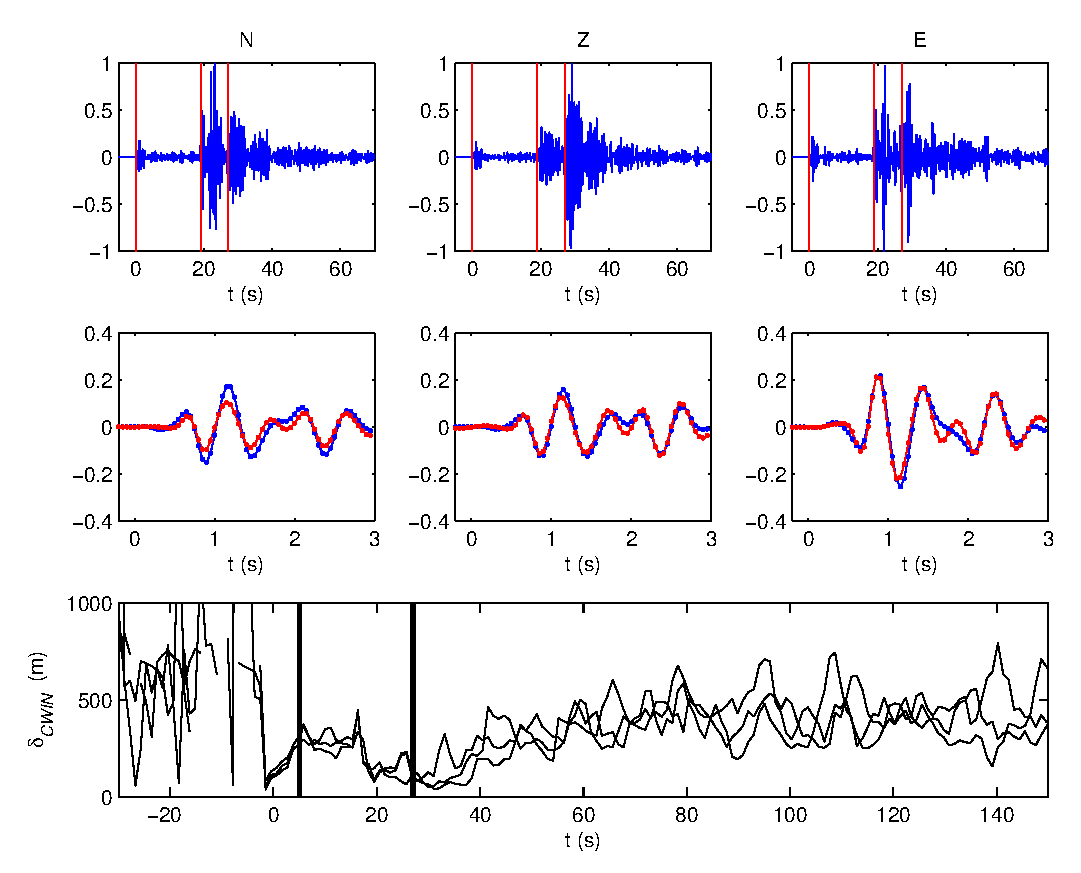
\includegraphics[width = 20pc]{diags/waves_and_CWIest.eps}} \\
\\
\\
\\
\\
\\
\\
\\
\\
\\
\\
\\
\\
\\
\\
\\
\\
\\
\end{tabular}
\caption{(a) Map of the South West Seismic Zone (SWSZ) illustrating the location of the Kalannie earthquake cluster,
the \cite{dr_Dawson08a} composite focal mechanism for the Kalannie events,
large historical events (focal mechanisms), observed seismicity between 1998 to 2007 (circles) and
Quaternary fault scarps (black lines) identified by \citet{dr_Clark09a}. The three available recording stations
MORW (162\,km), BLDU (67\,km) and KLBR (169\,km) are depicted with red triangles. Figure courtesy of
\citet{dr_Dawson08a} with minor modifications. (b) Example waveforms and CWI separation estimates
for the Kalannie events. The top row illustrates waveforms at station MORW for Event 1 normalised to maximum
amplitude and filtered between 1 and 2\,Hz for the three channels N,Z,E. Relative P, S and surface wave arrivals are also
indicated at 0, 19 and 27\,s, respectively. Middle row demonstrates similarity of first arrivals at station MORW for Events 1 and 2 in
the three channels. The bottom row shows the CWI separation estimates at MORW
as a function of sliding time window with width 5\,s for event pair 1 and 2. The three traces
represent different channels and the vertical black lines
enclose the region between $t=$5\,s and $t_{surf}$ that we consider for the remaining analysis.}
\label{fig:-Kalannie-map}
\end{figure}


\begin{figure}
\noindent\includegraphics[width = 20pc]{../../thesis_version2/diags/eq_location_simple/Kalannie_figs/Kalannie_Posteriors_timeclip_1to2Hz_tw5.eps}
\caption{Posterior functions $P_{ij}(\widetilde{\delta}_{t}|\widetilde{\delta}_{CWIN})$ for the Kalannie
event pairs $i$ and $j$. A
second $x$-axis is shown in separation units of meters for convenience.}
\label{fig:Kalannie-CWI-Posteriors}
\end{figure}

\begin{figure}
\begin{tabular}{ll}
(a) & (b) \\
\multirow{3}{*}{\noindent\includegraphics[width = 25pc]{../../thesis_version2/diags/eq_location_simple/KalannieNAB/Kalannie-CWI-NAB-1Dmarginals-withareas.eps}} & \multirow{2}{*}{\includegraphics[width = 10pc]{../../thesis_version2/diags/eq_location_simple/KalannieNAB/Kalannie_covariance.eps}}\\
&  \\
 & \\
 &
 \\
\\
\\
\\
\\
& (c) \\
&  \multirow{2}{*}{\includegraphics[width = 10pc]{../../thesis_version2/diags/eq_location_simple/KalannieNAB/Kalannie_correlation.eps}}\\
\\
\\
\\
\\
\\
\\
\\
\\
\\
\\
\end{tabular}
\caption{(a) One dimensional marginals for each of the six unknown Kalannie earthquake coordinates.
Labels $\hat{x}$, $\hat{y}$ and $\hat{z}$ refer to a local coordinate system with
origin corresponding to the event 1 location. Subscripts indicate the event number. Missing
parameters $\hat{y}_2$, $\hat{z}_2$ and $\hat{z}_3$ are set to 0 to remove rotational non-uniqueness without
loss of generality. Grey shaded regions illustrate the probability of each coordinate
being within 500\,m of the origin. The relative size of the shaded area
indicates that all event coordinates are likely within 500\,m of event 1
(see table \ref{tab:Kalannie-InversionRes} for actual areas). (b) Covariance and (c) correlation matrices
for the Kalannie earthquake location coordinates.
Different colours in the covariance matrix suggest different levels of resolvability between
coordinates. The off-diagonal structure of the correlation matrix indicates
a low level of trade-off between different coordinates.}
\label{fig:Kalannie-CWI-NAB-1Dmarginals}
\end{figure}


\begin{figure}
\noindent\includegraphics[width=20pc]{../../thesis_version2/diags/eq_location_simple/KalannieNAB/Kalannie_marginals2Dcont_param2_3.eps} \\
\caption{Marginal $P(\mathbf{e}_3) = P(\hat{x}_3,\hat{y}_3)$  for the location of event 3 normalised to unit volume.
We observe a clear maximum
near ($\hat{x}_3=290$\,m, $\hat{y}_3=300$\,m) and a local minimum near the origin. The black lines
enclose the 68\% confidence region. This figure suggests that events 3 and 1 (at origin) are close to one another but
not co-located and is consistent with the inversion results from the optimiser (magenta circle) and
MCMC (green circle).}
\label{fig:Kalannie-2Dmarginals_param23}
\end{figure}

\clearpage


\begin{table*}
\caption[InSAR source parameters for composite Kalannie mechanism]
{\cite{dr_Dawson08a} InSAR derived source parameters for a composite Kalannie mechanism with 1$\sigma$ uncertainties.
These parameters represent the point source which best explains the observed deformation at the surface. }
\label{tab-Dawson-Kalannie-results}
\begin{tabular}{ccccccc}
\hline
Long. ($^o$) & Lat. ($^o$) & Depth (km) & Mag. ($M_w$) & Strike ($^o$) & Dip ($^o$) & Rake ($^o$) \\
\hline
117.1700 & -30.1484 & 1.15 & 4.39 & 231.1 & 51.9 & 132.6 \\
$\pm$0.12\,km &  $\pm$0.10\,km & $\pm$0.08 & $\pm$0.06 & $\pm$12.1 & $\pm$6.2 & $\pm$11.1 \\
\hline
\end{tabular}
\end{table*}




\begin{table}
\caption[Kalannie earthquake magnitudes, seismic moments and dimensions]
{Estimated seismic moment $M_o$, moment magnitude $M_w$ and rupture diameter $2a$ for the
four Kalannie events using the local magnitude $M_L$ of the Geoscience Australia catalogue and conversion
formula discussed in text. In the case of the composite event (comp) we use the $M_w$ of \citet{dr_Dawson08a} and reverse
the calculations.}
\label{tab:Kalannie-eventsizes}
\begin{tabular}{c|ccccc}
\hline
Event & Date     & $M_L$ & $M_o$           & $M_w$   &  $2a$\\
      & (2005)   &       & ($10^{14}$\,Nm) &         &  (m)\\
\hline
1     &  21-Sept & 4     & $9.55$          & 3.9     & 694\\
2     &  21-Sept & 3.7   & $4.29$          & 3.7     & 531\\
3     &  22-Sept  & 4.1  & $12.47$         & 4       & 759\\
4     &  22-Sept  & 3.9  & $7.31$          & 3.8     & 635\\
comp  &  NA       & 4.6  & $48.4$          & 4.39    & 1192\\
\hline
\end{tabular}
\end{table}


\begin{table}
\caption{Inversion results for the Kalannie earthquake coordinates. The expected value $E[\bar{X}_i]$
and $var(\bar{X}_i)$ (the standard error of $E[\bar{X}_i]$) come from the Markov-chain Monte-Carlo approach, whereas
$\hat{x}_i^*$ result from the optimiser. The
outputs of both inversion procedures are consistent within the bounds of the standard error.
In the final column we show the probability of each event coordinate being within 500\,m of the origin $P_{500}$ (see grey
shaded regions of figure \ref{fig:Kalannie-CWI-NAB-1Dmarginals})}
\label{tab:Kalannie-InversionRes}
\renewcommand{\arraystretch}{1.5}
\begin{tabular}{c|cc|c|c}
\hline
parameter & $E[\bar{X}_i]$ &  $var(\bar{X}_i)$  & $\hat{x}_i^*$ & $P_{500}$\\
\hline
$\hat{x}_2$ & 348 & 220 & 329 & 0.76 \\
\hline
$\hat{x}_3$ & 156 & 433 & 307 & 0.68\\
$\hat{y}_3$ & 369 & 223 & 377 & 0.73\\
\hline
$\hat{x}_4$ & 102 & 402 & -124 & 0.76\\
$\hat{y}_4$ & 58 & 390 & 235 & 0.79\\
$\hat{z}_4$ & 315 & 224 & 201 & 0.81\\
\hline
\end{tabular}
\renewcommand{\arraystretch}{1}
\end{table}

\begin{table}
\caption{Separation estimates between Kalannie event pairs using
the optimisation and Markov-chain Monte-Carlo (MCMC) inversion
results. The separations are generally smaller
than the anticipated rupture size of each event (see table \ref{tab:Kalannie-eventsizes}) suggesting that
the events could rupture overlapping sections of the same fault. We have
more confidence in these separations than the pairwise CWI estimates because they
simultaneously incorporate all coda wave data.}
\label{tab:-KalannieRes-separations}
\begin{tabular}{c|cc}
\hline
Pair & Optimiser & MCMC \\
\hline
$\delta_{12}$ & 329 & 348 \\
$\delta_{13}$ & 486 & 401 \\
$\delta_{14}$ & 333 & 336 \\
$\delta_{23}$ & 378 & 416 \\
$\delta_{24}$ & 548 & 404 \\
$\delta_{34}$ & 496 & 446 \\
\hline
\end{tabular}
\end{table}

\end{document}

%%%%%%%%%%%%%%%%%%%%%%%%%%%%%%%%%%%%%%%%%%%%%%%%%%%%%%%%%%%%%%%

More Information and Advice:

%  SECTION HEADS

 ---------------
 Level 1 head

 Use the \section{} command to identify level 1 heads;
 type the appropriate head wording between the curly
 brackets, as shown below.

 Capitalize the first letter of each word (expect for
 prepositions, conjunctions, and articles that are
 three or fewer letters).

 Do not hyphenate level 1 heads. To break lines,
 type \protect\\ where you want the break to occur.
 AGU prefers the inverted triangle, breaking before
 prepositions, conjunctions, and articles, if possible.

An example:
\section{Level 1 Head: Introduction}

 ---------------
 Level 2 head

 Use the \subsection{} command to identify level 2 heads.

 Capitalize the first letter of each word (expect for
 prepositions, conjunctions, and articles that are
 three or fewer letters).

 Do not hyphenate level 1 heads. To break lines,
 type \protect\\ where you want the break to occur.
 AGU prefers the inverted triangle, breaking before
 prepositions, conjunctions, and articles, if possible.

\subsection{Level 2 Head} An example.

 ---------------
 Level 3 head

 Use the \subsubsection{} command to identify level 3 heads

 Capitalize only the first letter of the first word, acronyms,
 first letter of proper nouns, and first letter of first word
 after a colon.

 Hyphenation is permitted in level 3 heads, if needed.

\subsubsection{Level 3 Head} An example.

\subsubsubsection{Level 4 Head} An example.

%% ------------------------------------------------------------------------ %%
%
%  IN-TEXT LISTS
%
%% ------------------------------------------------------------------------ %%

% Do not use bulleted lists; enumerated lists are okay.
 \begin{enumerate}
 \item
 \item
 \item
 \end{enumerate}

%% ------------------------------------------------------------------------ %%
%
%  EQUATIONS
%
%% ------------------------------------------------------------------------ %%

% Single-line equations are centered.

 Math coded inside display math mode \[ ...\]
 will not be numbered e.g.:
 \[ x^2=y^2 + z^2\]

 Math coded inside \begin{equation} and \end{equation} will
 be automatically numbered e.g.:
 \begin{equation}
 x^2=y^2 + z^2
 \end{equation}

% IF YOU HAVE MULTI-LINE EQUATIONS, PLEASE
% BREAK THE EQUATIONS INTO TWO OR MORE LINES
% OF SINGLE COLUMN WIDTH (20 pc, 8.3 cm)
% using double backslashes (\\).

% To create multiline equations, use the
% \begin{eqnarray} and \end{eqnarray} environment
% as demonstrated below.
\begin{eqnarray}
  x_{1} & = & (x - x_{0}) \cos \Theta \nonumber \\
        && + (y - y_{0}) \sin \Theta  \nonumber \\
  y_{1} & = & -(x - x_{0}) \sin \Theta \nonumber \\
        && + (y - y_{0}) \cos \Theta.
\end{eqnarray}

If you don't want an equation number, use the star form:
\begin{eqnarray*}...\end{eqnarray*}

% Break each line at a sign of operation
% (+, -, etc.) if possible, with the sign of operation
% on the new line.

% Indent second and subsequent lines to align with
% the first character following the equal sign on the
% first line.

% Use an \hspace{} command to insert horizontal space
% into your equation if necessary. Place an appropriate
% unit of measure between the curly braces, e.g.
% \hspace{1in}; you may have to experiment to achieve
% the correct amount of space.

% There is another multiline equation environment:
% \begin{aguleftmath}...\end{aguleftmath}
% The equation is aligned left and the second line indents to
% the width of a paragraph indent (AGU style)


%% ------------------------------------------------------------------------ %%
%
%  EQUATION NUMBERING: COUNTER
%
%% ------------------------------------------------------------------------ %%

% You may change equation numbering by resetting
% the equation counter or by explicitly numbering
% an equation.

% To explicitly number an equation, type \eqnum{}
% (with the desired number between the brackets)
% after the \begin{equation} or \begin{eqnarray}
% command.  The \eqnum{} command will affect only
% the equation it appears with; LaTeX will number
% any equations appearing later in the manuscript
% according to the equation counter.
%
% To reset the equation counter, place the setcounter{equation}
% command in front of your equation(s).
%\setcounter{equation}{0}

% Set the equation counter to 0 if the next
% number needed is 1 or set it to 7 if the
% next number needed is 8, etc.
%
% The \setcounter{equation} command does affect
% equations appearing later in the manuscript.

% If you have a multiline equation that needs only
% one equation number, use a \nonumber command in
% front of the double backslashes (\\) as shown in
% the multiline equation above.



%%%%%%%%%%%%%%%%%%%%%%%%%%%%%%%%%%%%%%%%%%%%%%%%%%%%%%
%% Landscape figure and table examples
%
% ---------------
% Landscape (broadside) figure/table
% (These objects will not display properly in draft mode, use galley.)
%
% ONE-COLUMN landscape figure and table
%
% \begin{landscapefigure}
% \includegraphics[height=.75\mycolumnwidth,width=42pc]{samplefigure.eps}
% \caption{Caption text here}
% \end{landscapefigure}
%
% \begin{landscapetable}
% \caption{Caption text here}
% \begin{tabular*}{\hsize}{@{\extracolsep{\fill}}lcccc}
% \tableline
% ....
% \tableline\\
% \multicolumn5l{(a) Algorithms from Numerical Recipes}\\
% \end{tabular*}
% \tablenotetext{}{}
% \tablecomments{}
% \end{landscapetable}
%
% FULL-PAGE landscape figures and tables
%
% \begin{figure*}[p]
% \begin{landscapefigure*}
% illustration here
% \caption{caption here}
% \end{landscapefigure*}
% \end{figure*}
%
% \begin{table}[p]
% \begin{landscapetable*}
% \caption{}
% \begin{tabular*}{\textheight}{@{\extracolsep{\fill}}lccrrrcrrr}
% ....
% \end{tabular*}
% \begin{tablenotes}
% ...
% \end{tablenotes}
% \end{landscapetable*}
% \end{table}
%
